\documentclass[fleqn,10pt]{wlscirep} 

\usepackage{setspace}
\usepackage{lineno}
\doublespacing


%%%% (20 words or less)
\title{Genotypic variation in a foundation tree drives ecological network structure}

\author[1,2,*]{Matthew K. Lau}
\author[2]{Louis J. Lamit}
\author[3]{Rikke R. Naesbourg}
\author[4]{Stuart R. Borrett}
\author[5]{Matthew A. Bowker}
\author[1]{Thomas G. Whitham}

\affil[1]{Department of Biological Sciences and Merriam-Powell Center
  for Environmental Research, Northern Arizona University, Flagstaff,
  AZ 86011, USA}
\affil[2]{Harvard Forest, Harvard University, 324 N Main St,
  Petersham, MA 01366, USA}
\affil[3]{University of California Berkeley, Berkeley, CA, USA}
\affil[4]{Department of Biology and Marine Biology, University of
  North Carolina Wilmington, 601 South College Road, Wilmington, NC,
  28403, USA}
\affil[5]{School of Forestry, Northern Arizona University, Flagstaff,
  AZ 86011, USA}

\affil[*]{matthewklau@fas.harvard.edu}

%% \affil[+]{these authors contributed equally to this work}

\keywords{Keyword1, Keyword2, Keyword3}

\begin{abstract}

Biological evolution occurs in the context of complex networks of
interacting species in which natural selection defines the structure
of ecological networks. Fundamental to this evolutionary process is
the discovery of a genetic basis to ecological network
structure. Although previous work has demonstrated that tree genotype
contributes to interaction network structure at the scale of forest
stands, the contribution of tree genetics to localized interaction
networks at the scale of individual trees has not yet been
explored. To test the degree to which tree genetics can contribute to
network structure across scales from trees to stands, we conducted
quantitative modeling of interaction network for a community of
epiphytic lichens in a long-term experimental common garden of
genotyped trees of a foundation species (\textit{Populus
  angustifolia}). We found three main results: 1) Tree genotype
strongly contributed to network structure explaining over a third of
the variation in lichen interaction networks, 2) Multiple aspects of
interaction network structure varied in response to genotype,
including network size, the number of interactions, linkage density
and connectance, 3) At the stand scale, we also found signficant
modular structure of plant-lichen networks resulting in part from the
combination of trees of the same genotype tending to have similar
community compositions and supporting similar lichen interaction
networks dominated by positive interactions. These results support the
hypothesis that variation in ecological interaction networks can
result from genetically based variation in foundation
species. Although these results are for a community of sessile
organisms in close proximity to the tree, this study opens the
possibility for a genetic basis to both direct and indirect
interactions among species in complex communities.

\end{abstract}

\begin{document}

\flushbottom
\maketitle
% * <john.hammersley@gmail.com> 2015-02-09T12:07:31.197Z:
%
%  Click the title above to edit the author information and abstract
%
% ^ <thomas.whitham@nau.edu> 2018-03-02T21:05:44.603Z.
\thispagestyle{empty}

%% \noindent Please note: Abbreviations should be introduced at the
%% first mention in the main text – no abbreviations lists. Suggested
%% structure of main text (not enforced) is provided below.

\linenumbers

%%% For Submission to Nature Ecology and Evolution %%%
%%% https://www.nature.com/natecolevol/info


\section*{Introduction}


\section*{Methods}

\subsection*{Field observations in common garden and natural riparian forest stands}

The study was conducted along the Weber River, UT (USA), which is a
cottonwood (\textit{Populus} spp.) dominated riparian
ecosystem. Although two native species, \textit{Populus angustifolia}
(James) and \textit{Populus fremontii} (S. Watson), occur here and are
known to hybridize, only pure or advanced generation backcrosses of
\textit{P. angustifolia} were sampled in order to avoid the effect of
the hybridization between these two species.

A common garden was used to isolate the effect of tree genotype from
the effect of the localized microenvironment associated with each
individual and spatial autocorrelation. Asexually propagated clones of
genotyped \textit{P. angustifolia} individuals were obtained from wild
collections and planted randomly in a single field (0.025 km$^2$) at
the Ogden Nature Center, Ogden, UT in 1992. A total of thirteen
genotypes replicated between 3 and 8 times each, were chosen for
sampling. Genotype names were previously published
\cite{Martinsen}. Observations were made in the common garden in
October 2010 and May 2011.


\begin{figure}[ht]
\centering
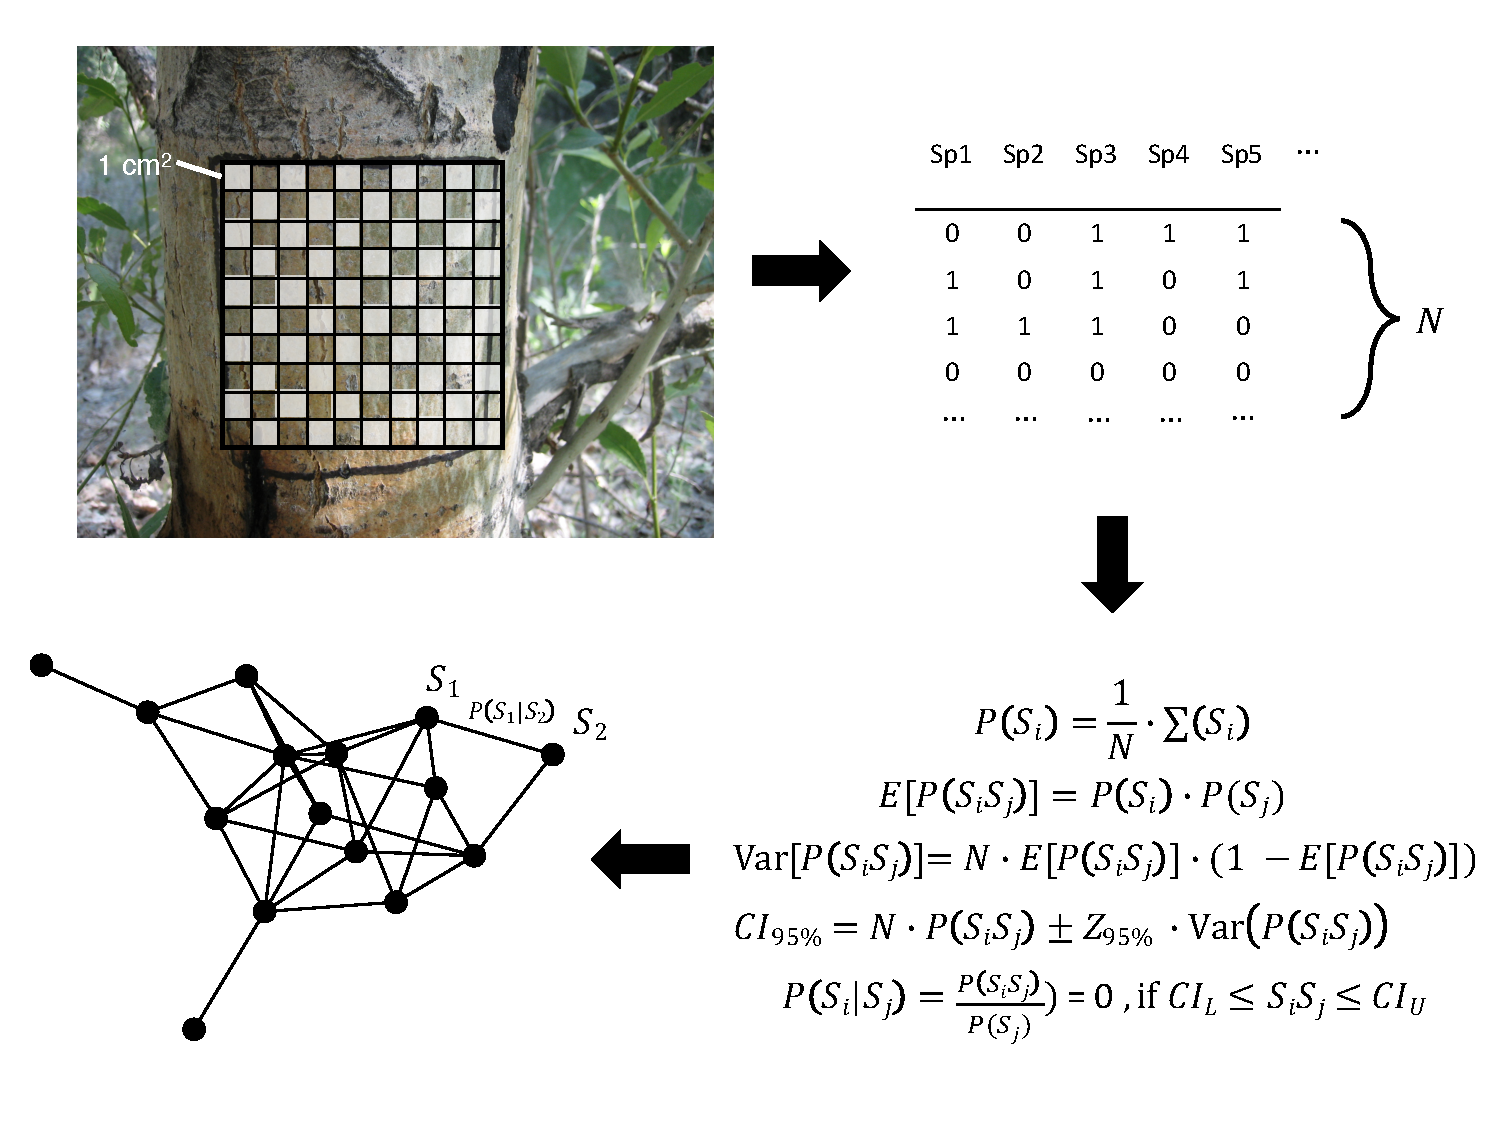
\includegraphics[width=\linewidth]{conet_method.pdf}
\caption{Lichen interaction networks were constructed by conducting
  field observations in 1 cm$^2$ cells within a 10 cm$^2$ grid on each
  tree using a checkerboard pattern (grey cells). Thus, a set of $N$
  total cell observations were recorded for each tree with the
  presence or absence of each species recorded for each cell. Applying
  a null-model based procedure \cite{Araujo2011}, we calculated and
  removed non-significant ($\alpha = 0.05$) co-occurrences to produce
  the network associated with an individual tree.}
\label{fig:conet_method}
\end{figure}



\section*{Results}


\begin{figure}[ht]
\centering
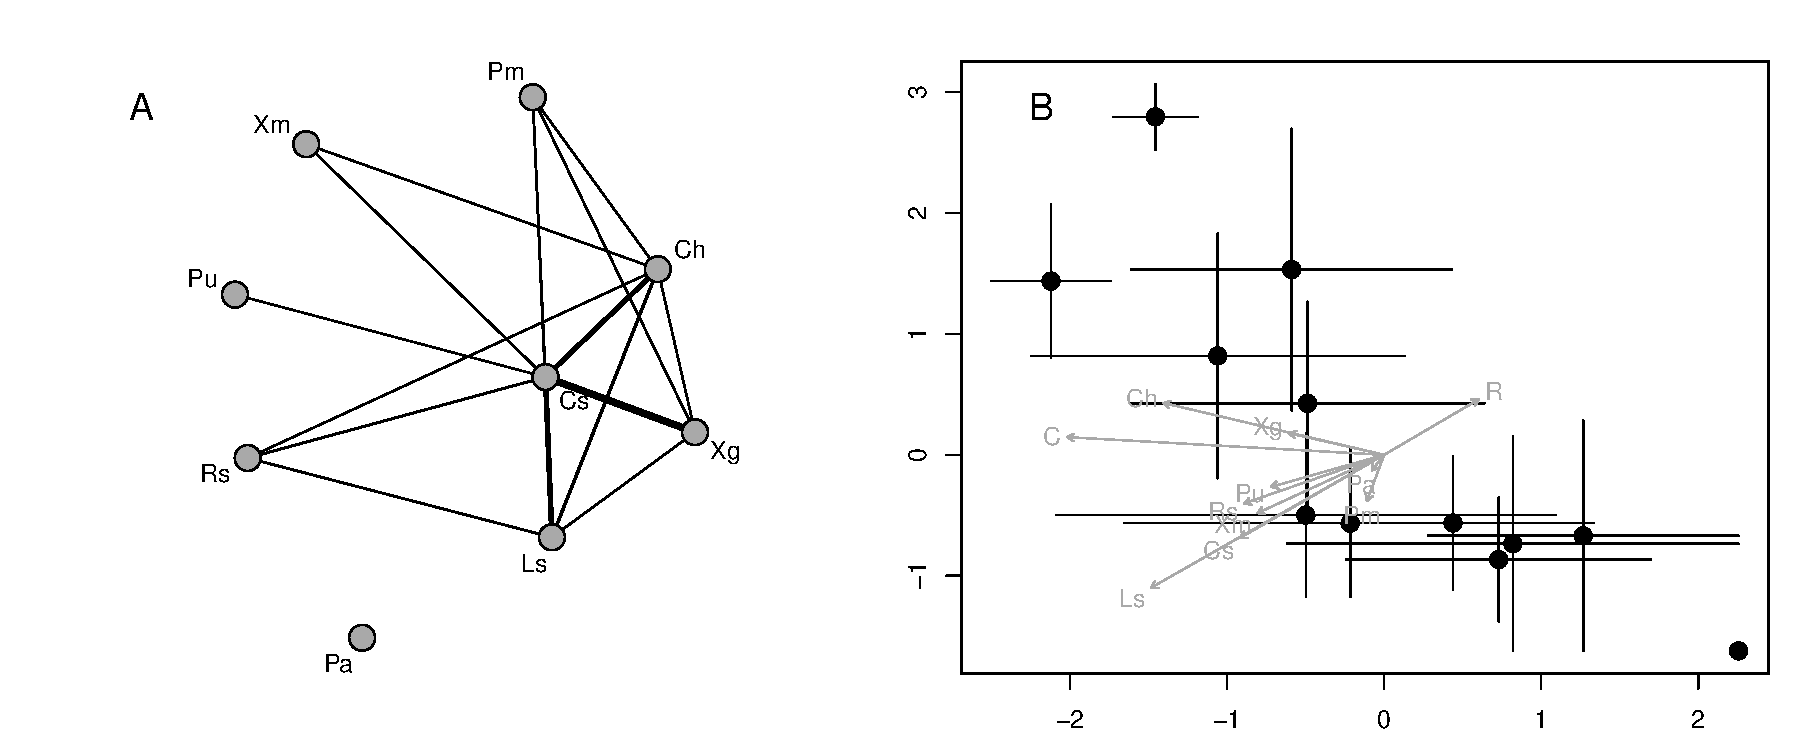
\includegraphics[width=\linewidth]{cn_chplot_onc.pdf}
\caption{Significant lichen interaction network structure resulting
  from tree genotypic variation was observed in the common garden. A)
  A network diagram showing significant interactions averaged over all
  trees shown as edges connecting lichen species shown as vertices. B)
  Genotype centroids (points) of NMDS ordinated lichen networks ($\pm$
  1 S.E.). Arrows show the magnitude and direction of correlation of
  the ordinated networks with tree bark roughness (R), network
  connectance and lichen species abundances (Xg =
  \textit{Xanthomendoza galericulata}, Xm = \textit{X. montana}, Ch =
  \textit{Caloplaca holocarpa}, Cs = \textit{Candelariella
    subdeflexa}, Rs = \textit{Rinodina} (unknown species), Ls =
  \textit{Lecanora} (unknown species), Pm = \textit{Phyciella
    melanchra}, Pa = \textit{Physcia adscendens}, Pu = \textit{Physcia
    undulata}).}
\label{fig:ch_plot}
\end{figure}

% latex table generated in R 3.4.4 by xtable 1.8-2 package
% Tue Nov 13 15:56:44 2018
\begin{table}[ht]
\centering
\begin{tabular}{llll}
  \hline
Response & Predictor & p-value & H2 \\ 
  \hline
Percent Lichen Cover & Tree Genotype & 0.0356 & 0.17 \\ 
  Lichen Species Richness & Tree Genotype & 0.1443 & 0.1 \\ 
  Percent Rough Bark & Tree Genotype & 8e-04 & 0.38 \\ 
  Lichen Network & Genotype & 0.0431 & 0.17 \\ 
  Number of Network Links & Genotype & 0.0796 & 0.15 \\ 
  Network Centrality & Genotype & 0.1351 & 0.12 \\ 
   &  &  &  \\ 
   &  &  &  \\ 
   &  &  &  \\ 
   \hline
\end{tabular}
\caption{Genotypic effects of cottonwood trees on the associated lichen community.} 
\label{tab:h2_table}
\end{table}


%% \begin{figure}[ht]
%% \centering
%% \includegraphics[width=\linewidth]{}
%% \caption{}
%% \label{fig:}
%% \end{figure}

\begin{figure}[ht]
\centering
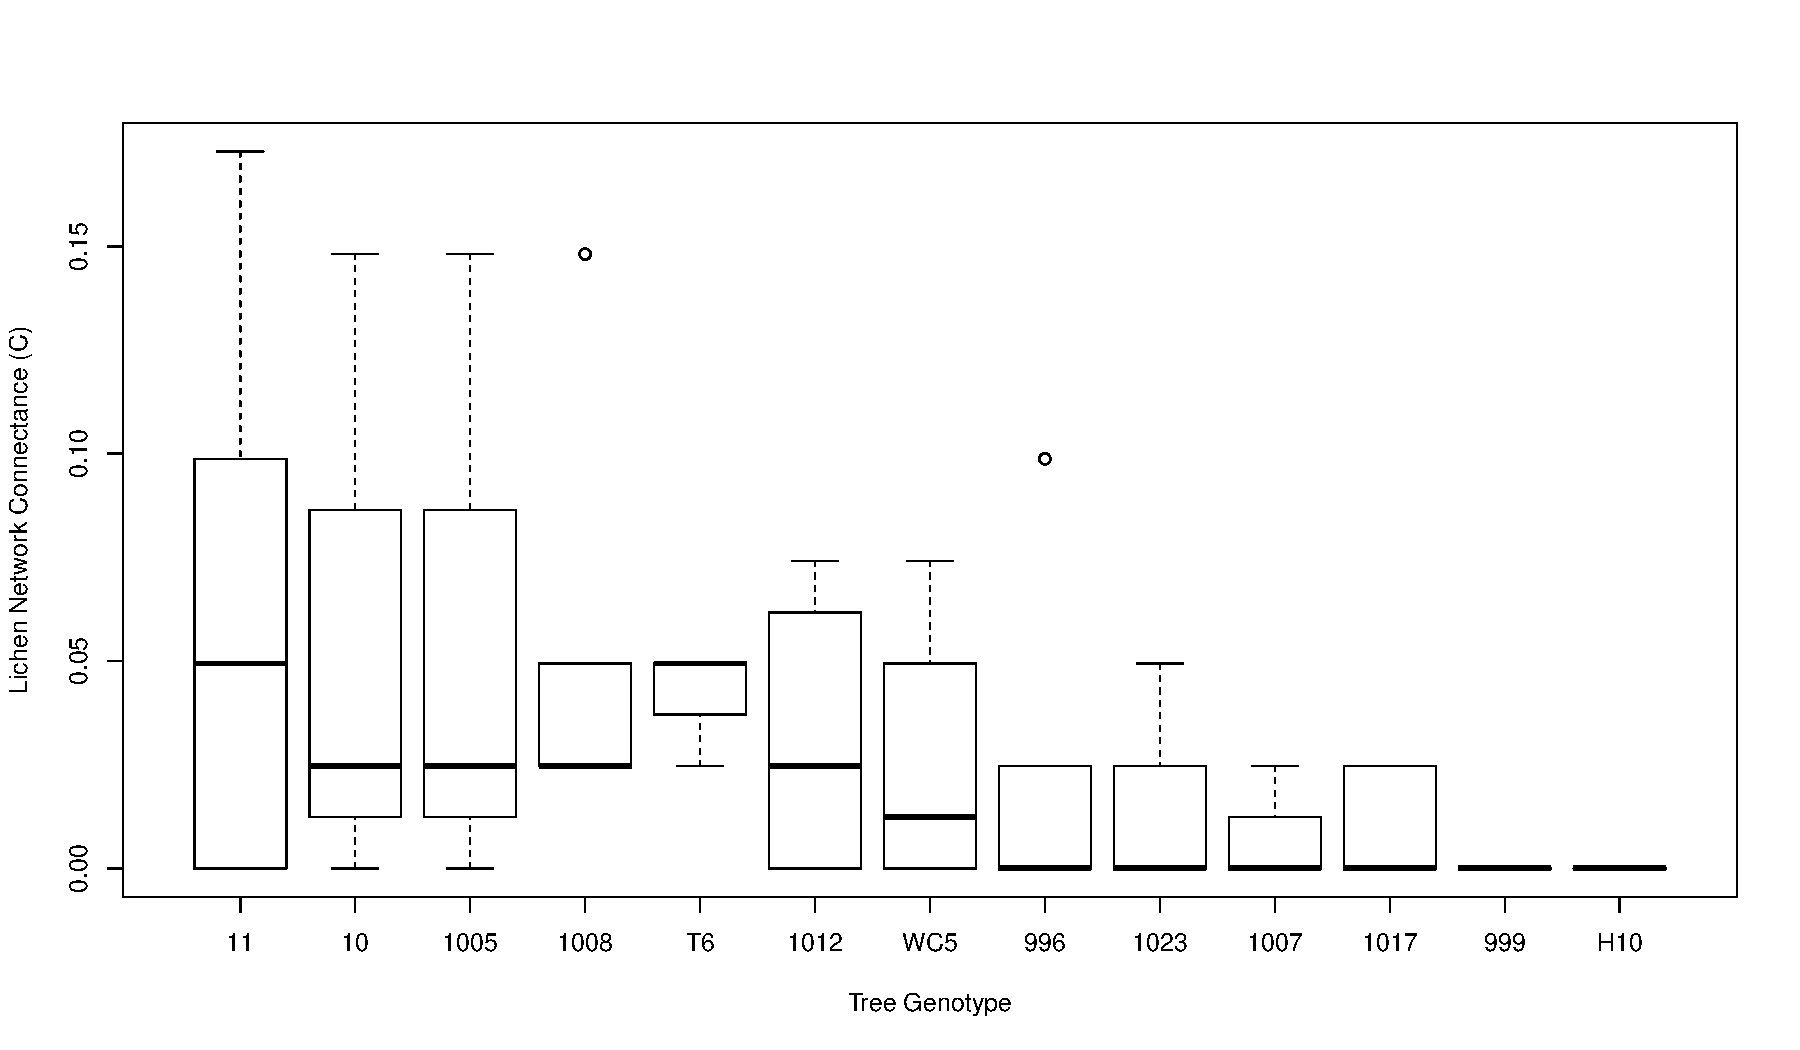
\includegraphics[width=\linewidth]{connect_geno.pdf}
\caption{Connectance significantly varied among genotypes.}
\label{fig:connect}
\end{figure}


\begin{figure}
\centering
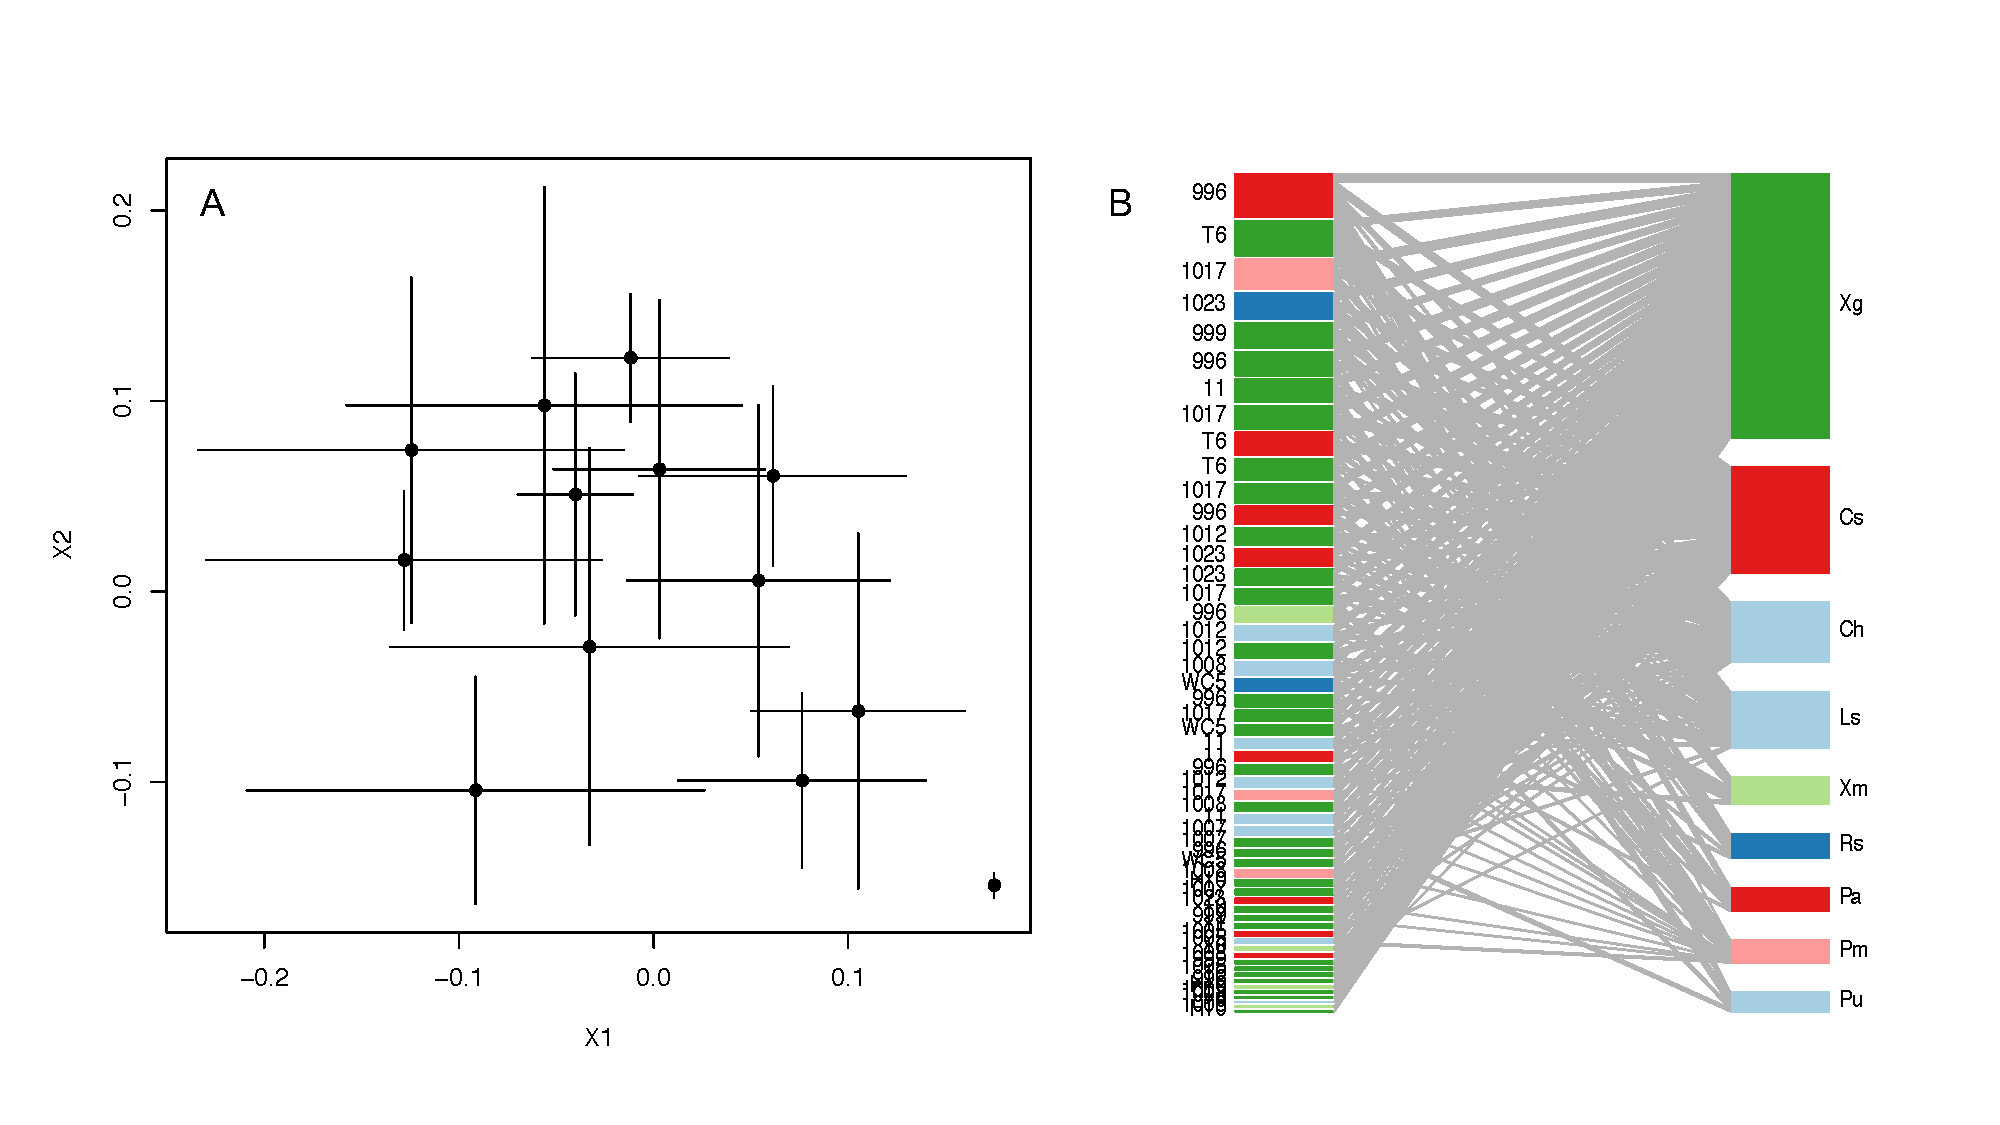
\includegraphics[width = \textwidth]{lcn_com_bpnet.pdf}
%% 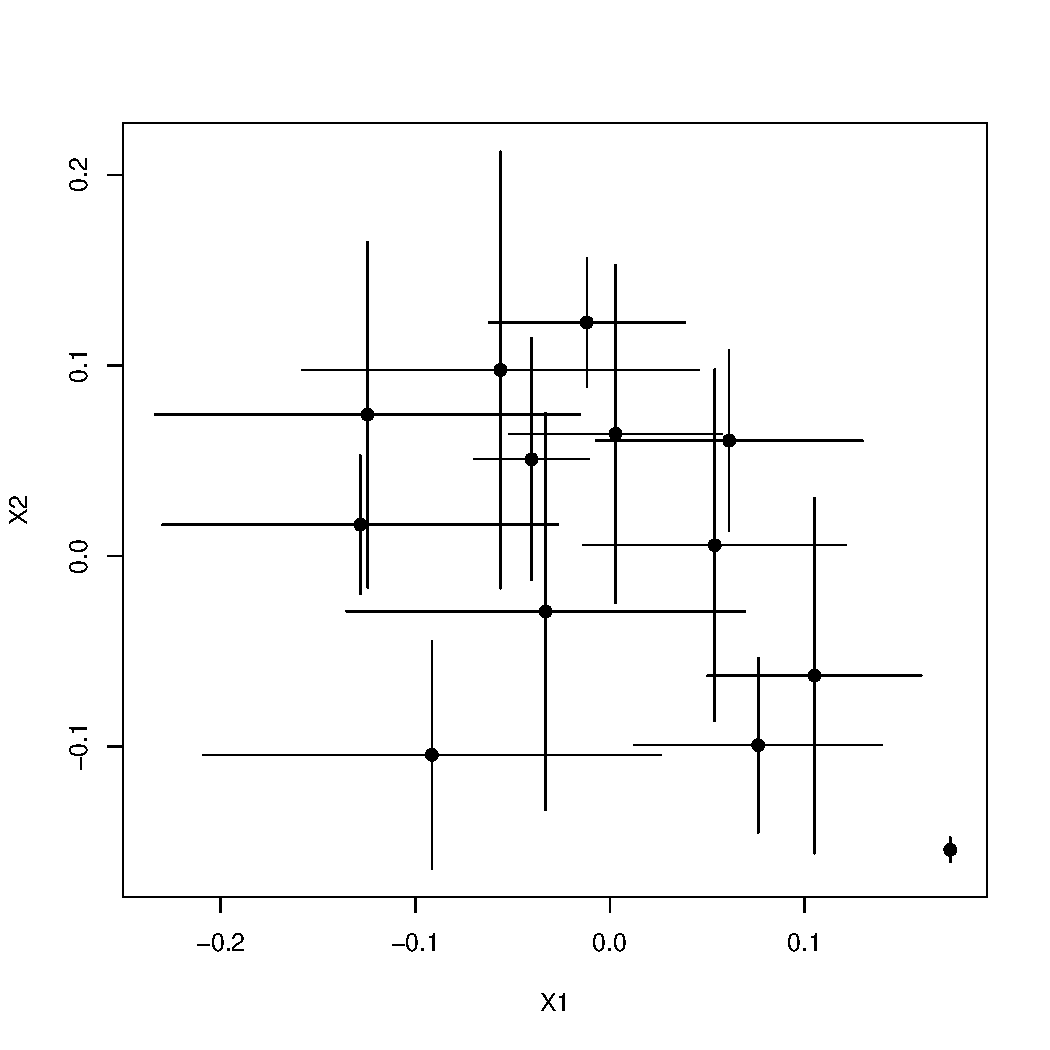
\includegraphics[width = 0.4\textwidth]{chp_com_onc.pdf}
%% 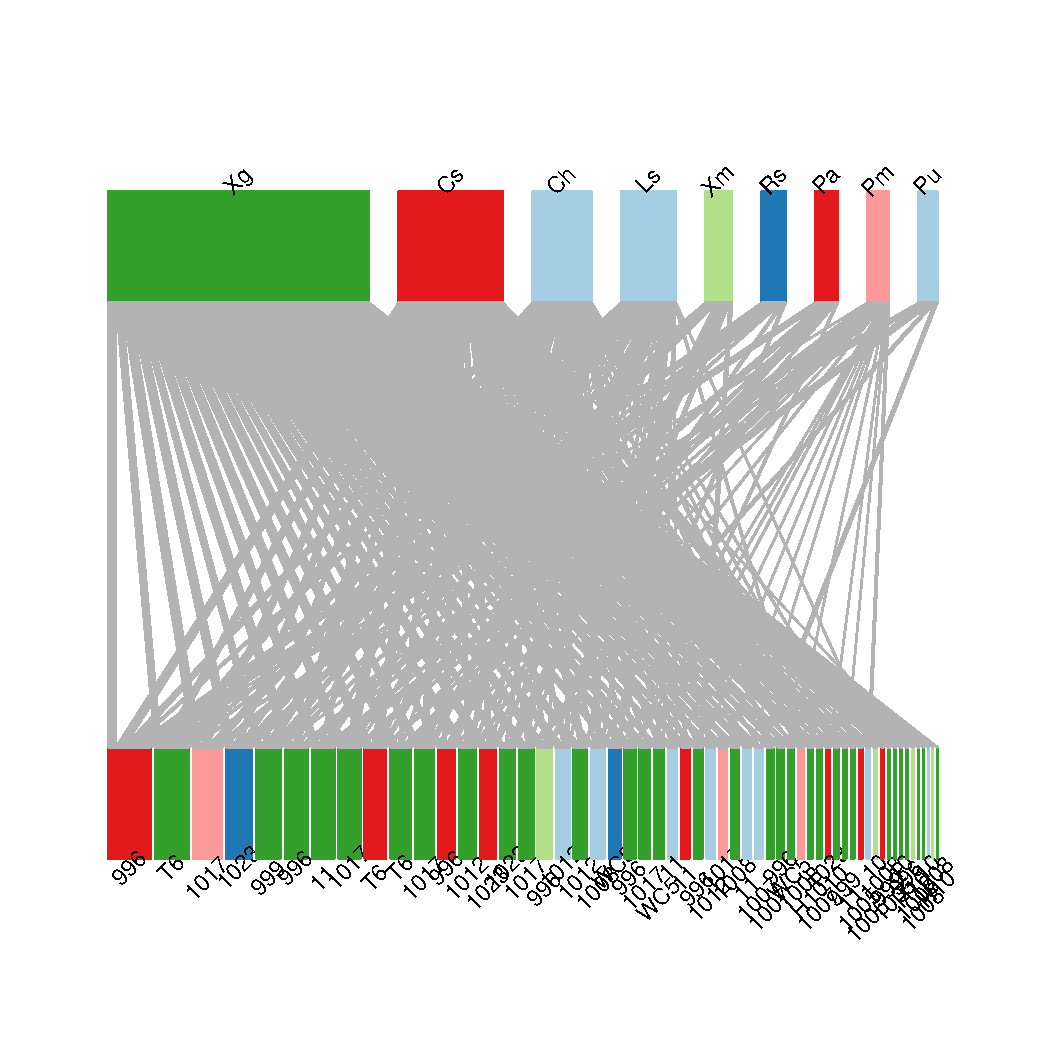
\includegraphics[width = 0.4\textwidth, angle = -90]{bp_net_onc.pdf}
\caption{Tree genotype varition in lichen community composition also
  contributed to genotype-species bipartite intreraction network
  structure at the scale of the common garden stand. A) Plot of the
  ordinated community composition scores shown as centroids ($\pm$ 1
  S.E.). B) Bipartite interaction network based on the occurrences of
  lichen on individual cottonwood trees in the common garden. Edges
  connecting trees to lichen are scaled by the relative abundance of
  lichen. Nodes of lichen and trees are colored by their module
  membership.}
\label{fig:bpnet}
\end{figure}





\subsection*{Network Response to Tree Variation}


\subsection*{Genetic Structure Generates Forest Scale Network Structure}


\clearpage
\newpage


\section*{Discussion}

\bibliography{lichen_network_genetics}

%% \noindent LaTeX formats cites and references automatically using
%% the bibliography records in your .bib file, which you can edit via the
%% project menu. Use the cite command for an inline cite, e.g.
%% \cite{Figueredo:2009dg}.

\section*{Acknowledgments} 

This work was supported by the National Science Foundation grant
(DEB-0425908) and Integrative Graduate Research Traineeship (IGERT)
fellowships for M.L. and L.L. The Ogden Nature Center staff helped to
maintain the common gardens. Lichen sampling was supported by Todd
Wojtowicz, Luke Evans and David Solance Smith.


\section*{Author contributions statement}

M.L. and L.L. conceived the study, M.L. and L.L. conducted the field
work, R.N.  assisted in lichen identifications, M.L. wrote the first
draft of the manuscript, S.B. and T.W. contributed substantively to
the conceptual development, T.W. established the common garden. All
authors contributed to revisions of the manuscript.

\section*{Additional information}

%% To include, in this order: \textbf{Accession codes} (where
%% applicable); \textbf{Competing financial interests} (mandatory
%% statement).

%% The corresponding author is responsible for submitting a
%% \href{http://www.nature.com/srep/policies/index.html#competing}{competing
%% financial interests statement} on behalf of all authors of the
%% paper. This statement must be included in the submitted article
%% file.


\clearpage
\newpage


%% Figures and tables can be referenced in LaTeX using the ref command, e.g. Figure \ref{fig:stream} and Table \ref{tab:example}.

\end{document}
